\section{Payment component}
\label{sec:payment_component}
Until now it has been shown how it works internally handling payments. Let's see how to mask this complexity in integrating the payment system in x-commerce.
\newline
All logic of the payment is hidden in the component \emph{payment-braintree}.
\newline
Following is illustrated in detail the use of the component \emph{payment-braintree}:
\begin{lstlisting}[language=html]
<payment-braintree id="braintree"></payment-braintree>
\end{lstlisting}
So just import this tag to integrate into your system the payments system. All this thanks to the web components.
\newline
The result of having imported this component is the following:
\begin{figure}[htb]
 \centering
 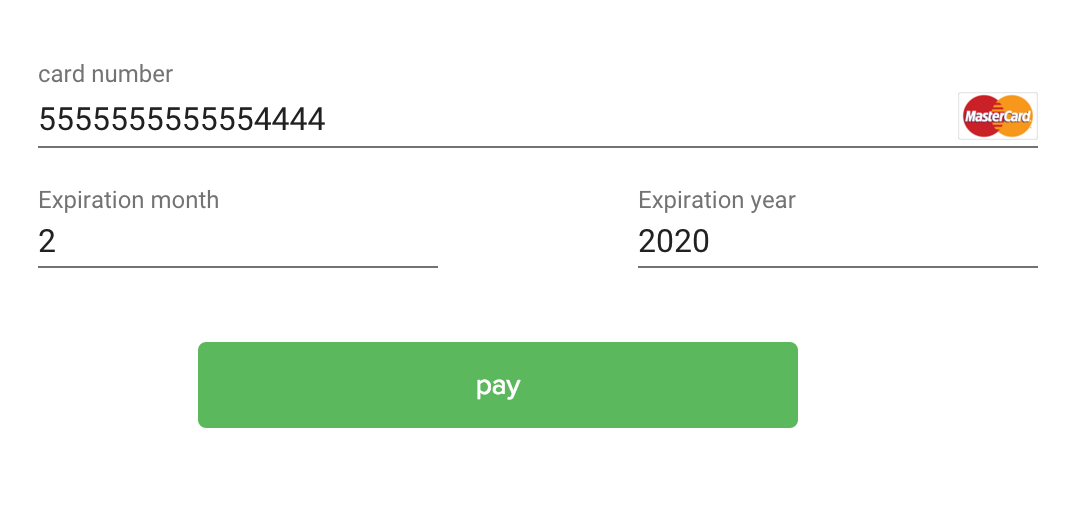
\includegraphics[width=0.8\linewidth]{images/chapter5/braintree1.png}\hfill
 \caption[Braintree form]{Braintree form for payment}
 \label{fig:brintree_form1}
\end{figure}
The management of payments with Stripe everything works the same way but does not implement the logic of gestone task when paying anadato bad. In fact, to import the payment form stripe just include the following tag:
\begin{lstlisting}[language=html]
<payment-stripe id="stripe"></payment-stripe>
\end{lstlisting}
The result of having imported this component is the following:
\begin{figure}[htb]
 \centering
 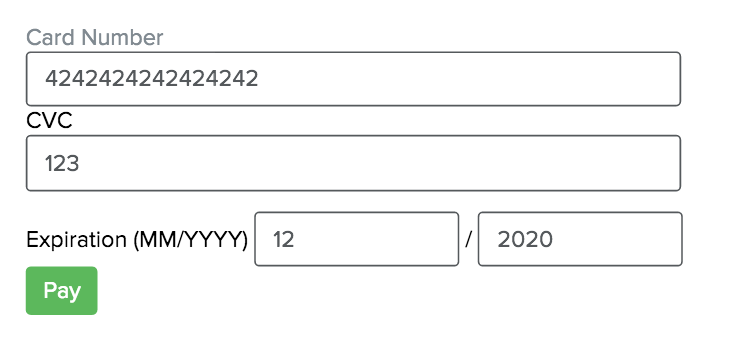
\includegraphics[width=0.8\linewidth]{images/chapter5/stripe1.png}\hfill
 \caption[Stripe form]{Stripe form for payment}
 \label{fig:brintree_form1}
\end{figure}